\documentclass[oneside]{book}
\usepackage{color}
\usepackage{fancyhdr}
\usepackage{geometry}
\usepackage{graphicx}
\usepackage{ifthen}
\usepackage{makeidx}
\usepackage{moreverb}
\usepackage{times}
\usepackage{verbatim}
\usepackage{hyperref}

\geometry{letterpaper,margin=1in}

\pagestyle{fancy}
\fancyhf{}
\lhead{\bf\nouppercase\rightmark}
\rhead{\bf Page\space\thepage}

\newenvironment{entry}%
  {\begin{list}{}{\renewcommand{\makelabel}[1]%
    {\parbox[b]{\labelwidth}{\makebox[0pt][l]{\textbf{##1}}\\}}%
    \setlength{\labelwidth}{1em}%
    \setlength{\labelsep}{1em}%
    \setlength{\leftmargin}{2em}%
    \setlength{\topsep}{\medskipamount}%
    \setlength{\itemsep}{\medskipamount}%
    \setlength{\parsep}{\medskipamount}%
    \setlength{\listparindent}{0pt}}}
  {\end{list}}
\newenvironment{indented}%
  {\begin{list}{}{\setlength{\leftmargin}{2em}}%
    \setlength{\itemsep}{\medskipamount}%
    \setlength{\parsep}{\medskipamount}%
    \setlength{\listparindent}{0pt}\item}
  {\end{list}}

\let\keepttfamily\ttfamily
\def\ttfamily{\color{blue}\keepttfamily}
\def\listinglabel#1{\llap
  {\scriptsize\color{black}\the#1}\hskip\listingoffset\relax}

\newcommand\idx[2][xxx]{%
  \ifthenelse{\equal{#1}{xxx}}{\index{#2@\texttt{#2}}}%
  {\index{#2@\texttt{#2}}\index{#1!#2@\texttt{#2}}}}

\bibliographystyle{lalapps}

\makeindex

\begin{document}

\frontmatter

\title{LALApps --- LSC Algorithm Library Applications}
\author{Contact: Jolien Creighton \texttt{jolien@gravity.phys.uwm.edu}}
\maketitle

\thispagestyle{empty}
\chapter*{Authors}
\verbatiminput{AUTHORS}

\tableofcontents

\mainmatter

\chapter{LALApps utilities}

Several utilities (macros, global variables, and functions) are provided to
assist in writing programs in LALApps, and for maintaining a standard
look-and-feel.  This chapter describes these utilities and concludes with
the listing of an example program.

\newpage
\section{Header \texttt{lalapps.h}}
\label{header:lalapps}

\begin{indented}
Provides utilities for writing programs for LALApps.

Several macros, global variables, and function prototypes are given that will
assist in writing LALApps programs, and will aid in maintaining a standard
look-and-feel.

To use these utilities, include the header \verb$lalapps.h$ and make sure the
program links to the object \verb$lalapps.o$.
\end{indented}

\newpage
\subsection{Function \texttt{set\_debug\_level}}
\label{function:set-debug-level}
\idx[Function]{set\_debug\_level}
\index{Debug Level}
\idx[Variable]{lalDebugLevel}
\idx[Debug Level]{lalDebugLevel}
\idx[Debug Level]{NDEBUG}
\idx[Debug Level]{ERROR}
\idx[Debug Level]{WARNING}
\idx[Debug Level]{INFO}
\idx[Debug Level]{TRACE}
\idx[Debug Level]{MEMINFO}
\idx[Debug Level]{MEMDBG}
\idx[Debug Level]{MSGLVL1}
\idx[Debug Level]{MSGLVL2}
\idx[Debug Level]{MSGLVL3}
\idx[Debug Level]{ALLDBG}
\idx[Environment]{LAL\_DEBUG\_LEVEL}

\begin{entry}

\item[Name]

\verb$set_debug_level$ --- sets the LAL debug level

\item[Synopsis]

\begin{verbatim}
#include <lalapps.h>
extern int lalDebugLevel;
int set_debug_level( const char *s );
\end{verbatim}

\item[Description]

The function \verb$set_debug_level$ sets the LAL debug level to a value
determined by the string \verb$s$, which can be an absolute debug level
(a string representing an integer) or a string of LAL debug level flags.
Allowed flags are:
\begin{indented}
\begin{entry}
\item[NDEBUG]
  No debugging information is printed and memory debugging code is disabled.
\item[ERROR]
  Error messages are printed.
\item[WARNING]
  Warning messages are printed.
\item[INFO]
  Information messages are printed.
\item[TRACE]
  Function call tracing messages are printed.
\item[MEMINFO]
  Memory allocation information messages are printed.
\item[MEMDBG]
  Debugging of memory allocation routines is enabled bug no messages are
  printed.
\end{entry}
\end{indented}
The following pre-defined composite levels are available:
\begin{indented}
\begin{entry}
\item[MSGLVL1]
  Equivalent to \verb$ERROR$.
\item[MSGLVL2]
  Equivalent to \verb$ERROR | WARNING$.
\item[MSGLVL3]
  Equivalent to \verb$ERROR | WARNING | INFO$.
\item[ALLDBG]
  All debugging messages are printed.
\end{entry}
\end{indented}

If the argument to \verb$set_debug_level$ is \verb$NULL$, then the string
stored in the environment variable \verb$LAL_DEBUG_LEVEL$ is used.  If this
environment is not defined, or if no flags or values are specified in the
string, the debug level is set to 0, which is equivalent to \verb$NDEBUG$.
(This is also the default value for \verb$lalDebugLevel$ unless it is set to
some other value.)

For example, the statement
\begin{indented}
\verb$set_debug_level( "ERROR | INFO" );$
\end{indented}
will set the debug level so that error and information messages are printed
(but not warning messages).  Another example is the statement
\begin{indented}
\verb$set_debug_level( "2" );$
\end{indented}
which would set the debug level to 2 (warning messages are printed).

\item[Return Value]

The return value is the (integer) debug level that is assigned to
\verb$lalDebugLevel$.

\item[Environment]
\leavevmode
\begin{entry}
\item[\texttt{LAL\_DEBUG\_LEVEL}]
  Default LAL debug level string to use.
\end{entry}

\end{entry}

\newpage
\subsection{Function \texttt{clear\_status}}
\label{function:clear-status}
\idx[Function]{clear\_status}
\idx[Variable]{blank\_status}

\begin{entry}

\item[Name]
\verb$clear_status$ --- clears the LAL status structure after a failed LAL
function call

\item[Synopsis]
\begin{verbatim}
#include <lalapps.h>
extern const LALStatus blank_status;
int clear_status( LALStatus *status );
\end{verbatim}

\item[Description]
Clears the LAL status structure and iteratively frees attatched (sic) any
linked status structures.  This is to be used after a failed LAL function
call to restore the status structure to a useable form.  The structure
\verb$blank_status$ contains a blank status structure that can be used to
initialize a status structure in the program.

\item[Example]

The following program calls a routine \verb$LALFailUnlessNegative$ twice,
once with a positive argument (which causes the routine to fail) and once
with a negative argument (which causes the routine to pass).  The function
\verb$clear_status$ is used to clean up the status structure after the
failure and the constant structure \verb$blank_status$ is used to initialize
the status structure.

\begin{indented}
\begin{verbatim}
#include <lalapps.h>
#include <lal/LALStdlib.h>

extern const LALStatus blank_status;

void LALFailUnlessNegative( LALStatus *status, INT4 n )
{
  INITSTATUS( status, "LALFail", "$Id$" );
  ATTATCHSTATUSPTR( status );
  ASSERT( n, status, 1, "Non-negative n" );
  if ( n > 0 )
  {
    TRY( LALFailUnlessNegative( status->statusPtr, n - 1 ), status );
  }
  DETATCHSTATUSPTR( status );
  RETURN( status );
}

int main( void )
{
  LALStatus status = blank_status;
  LALFailUnlessNegative( &status, 5 );
  clear_status( &status );
  LALFailUnlessNegative( &status, -2 );
  return status.statusCode;
}
\end{verbatim}
\end{indented}

\end{entry}


\newpage
\subsection{Macro \texttt{RCSID}}
\label{macro:RCSID}
\idx[Macro]{RCSID}
\idx[Variable]{rcsid}

\begin{entry}

\item[Name]

\verb$RCSID$ --- set the RCS Id variable

\item[Synopsis]

\begin{verbatim}
#include <lalapps.h>
#ifndef RCSID
#define RCSID( id ) static volatile const char *rcsid = (id)
#endif
\end{verbatim}

\item[Description]

\verb$RCSID$ sets the static (i.e., internal-linkage) variable \verb$rcsid$
to the RCS Id string, \$\relax Id\$, which is given as the argument \verb$id$.
The string \$\relax Id\$ is expanded by RCS to contain the identification of
the source file along with its revision number.
For example:
\begin{indented}
\verb+RCSID("$+\verb+Id+\verb+$");+
\end{indented}

\end{entry}

\newpage
\subsection{Macro \texttt{PRINT\_VERSION}}
\label{macro:PRINT-VERSION}
\idx[Macro]{PRINT\_VERSION}

\begin{entry}

\item[Name]
\verb$PRINT_VERSION$ --- prints the LALApps version of the program

\item[Synopsis]
\begin{verbatim}
#include <lalapps.h>
static volatile const char *rcsid="$Id$";
#ifndef PRINT_VERSION
#define PRINT_VERSION( program ) \
  fprintf( stderr, PACKAGE " %s version " VERSION "\n%s\n", program, rcsid )
#endif
\end{verbatim}

\item[Description]
\verb$PRINT_VERSION$ prints the version information for \verb$program$ in a
standard format, along with the RCS Id information.  For example, for the
program \verb$lalapps_hello$, the version information
\begin{indented}
\verb+lalapps hello version 0.1+\\
\verb+$+\verb+Id+\verb+$+
\end{indented}
is printed with the command \verb$lalapps_hello -V$.  The source code to
print this is
\begin{indented}
\verb$PRINT_VERSION( "hello" );$
\end{indented}

Note that \verb$PRINT_VERSION$ requires the string variable \verb$rcsid$ to be
set.

\end{entry}

\newpage
\subsection{Macro \texttt{LAL\_CALL}}
\label{macro:LAL-CALL}
\idx[Macro]{LAL\_CALL}
\idx[Variable]{vrblvl}
\idx[Function]{lal\_errhandler}
\idx[Type]{lal\_errhandler\_t}
\index{Error Handler}
\idx[Error Handler]{LAL\_ERR\_DFLT}
\idx[Error Handler]{LAL\_ERR\_ABRT}
\idx[Error Handler]{LAL\_ERR\_EXIT}
\idx[Error Handler]{LAL\_ERR\_RTRN}

\begin{entry}

\item[Name]
\verb$LAL_CALL$ --- call a LAL routine and handle any errors

\item[Synopsis]
\begin{verbatim}
#include <lalapps.h>

extern int vrblvl;
extern int ( *lal_errhandler )( LALStatus *stat, const char *func,
    const char *file, const int line, volatile const char *id );
extern lal_errhandler_t lal_errhandler;

static volatile const char *rcsid="$Id$";

#ifndef LAL_CALL
#define LAL_CALL( function, statusptr ) \
  ((function),lal_errhandler(statusptr,#function,__FILE__,__LINE__,rcsid))
#endif
\end{verbatim}

\item[Description]
\verb$LAL_CALL$ executes the LAL function \verb$function$ and executes the
error handler \verb$lal_errhandler$, which examines the status structure
\verb$statusptr$ to see if an error occurred.  Typically the error handler
will return with value 0 if there was no error; otherwise it will print a trace
of the execution stack and then perform a specific action.  The action
performed depends on the error handler, which can be set to one of the
following:
\begin{indented}
\begin{entry}
\item[\texttt{LAL\_ERR\_DFLT}]
  The default error handler (same as \verb$LAL_ERR_ABRT$).
\item[\texttt{LAL\_ERR\_ABRT}]
  Raises \verb$SIGABRT$ if there is an error.
\item[\texttt{LAL\_ERR\_EXIT}]
  Exits with the returned status code if there is an error.
\item[\texttt{LAL\_ERR\_RTRN}]
  Returns the status code.
\end{entry}
\end{indented}

Note that \verb$LAL_CALL$ requires the string variable \verb$rcsid$ to be set.

\item[Return Value]
If \verb$LAL_CALL$ returns (rather than terminating execution), the return
value is equal to the status code returned by the LAL function.

\item[Example]
The following example program illustrates the use of \verb$LAL_CALL$.
The routine \verb$LALInvert$ is called incorrectly twice.  The first time
the division by zero error is caught.  The second time, the unexpected null
pointer error is not caught and the default error handler aborts the program.
\begin{indented}
\begin{verbatim}
#include <stdlib.h>
#include <lalapps.h>
#include <lal/LALStdlib.h>

RCSID( "$Id$" );

extern int vrblvl;
extern const LALStatus blank_status;

void LALInvert( LALStatus *status, REAL4 *y, REAL4 x )
{
  INITSTATUS( status, "LALInvert", rcsid );
  ASSERT( y, status, 1, "Null pointer" );
  if ( input == 0 )
  {
    ABORT( status, 1, "Division by zero" );
  }
  *y = 1 / x;
  RETURN( status );
}

int main( void )
{
  LALStatus status = blank_status;
  REAL4 x;
  int code;

  vrblvl = 1;

  lal_errhandler = LAL_ERR_RTRN;
  code = LAL_CALL( LALInvert( &status, &x, 0 ), &status );
  if ( code == 2 )
  {
    puts( "division by zero" );
    clear_status( &status );
  }
  else if ( code )
  {
    exit( code );
  }

  lal_errhandler = LAL_ERR_DFLT;
  LAL_CALL( LALInvert( &status, NULL, 1 ), &status );

  return 0;
}
\end{verbatim}
\end{indented}

\end{entry}

\newpage
\section{Source \texttt{hello.c}}
\label{source:hello.c}
\idx[Source]{hello.c}

\begin{indented}
This is the source code for the program \verb$lalapps_hello$:

\listinginput[10]{1}{hello.c}
\end{indented}

\chapter{LALApps programs}

This chapter describes the programs that are part of the LALApps package.


%%
%% INCLUDE YOUR DOCUMENTATION BELOW
%%

\chapter{Package \texttt{hello}}

This is an example package that illustrates how to write and document LAL
code.  This pacakage contains a routine that prints ``hello, LSC!''

\newpage\input{LALHelloH}

\section{Program \texttt{lalapps\_animate}}
\label{program:lalapps-animate}
\idx[Program]{lalapps\_animate}

\begin{entry}

\item[Name]
\verb$lal_animate$ --- produces an animated display showing the time
series output of a selected channel in a lower window, and a simultaneously
calculated FFT power spectrum in the upper window

\item[Synopsis]
\verb$lal_animate$ [\verb$--help$] [\verb$--channel$ \textit{name}] 
[\verb$--duration$ \textit{secs}] [\verb$--epoch$ \textit{sec}
\textit{nsec}] [\verb$--framedir$ \textit{dirname}] 
[\verb$--highpass$ \textit{freq} \textit{attenuation}]
[\verb$--numpts$ \textit{npoints}] $|$ xmgr -pipe

%              "    --help                Print this help message\n" \
%              "    --channel name        Name of frame channel\n" \
%              "   [--duration secs]      How many seconds to look at\n"\
%              "   [--epoch sec nsec]     The starting epoch\n"\
%              "   [--framedir dirname]   Directory containing frame files\n"\
%              "   [--highpass freq attenuation]  High-pass filter parameters \n"\
%              "   [--numpts npoints]     Points per graph displayed\n"

\item[Description]
\verb$lal_animate$ produces an animated display showing the time
series output of a selected channel in a lower window, and a simultaneously
calculated FFT power spectrum in the upper window.  The output from
this program must be piped into the graphing program \texttt{xmgr}.

\item[Options]\leavevmode
\begin{entry}
\item[\texttt{--help}]
Print a help message.
\item[\texttt{--channel} \textit{name}]
Name of frame channel
\item[\texttt{--duration} \textit{secs}] 
How many seconds to look at
\item[\texttt{--epoch} \textit{sec} \textit{nsec}] 
Starting epoch
\item[\texttt{--framedir} \textit{dirname}] 
Directory containing frame files
\item[\texttt{--highpass} \textit{freq} \textit{attenuation}]
High-pass filter parameters
\item[\texttt{--numpts} \textit{npoints}]
Points per graph to display
\end{entry}

\item[Example]
To run the program,  type:
\begin{verbatim}
lalapps_animate --channel H2:LSC-AS_Q --framedir ./h1 --numpts 16384 \
--epoch 693768272 0 --duration 1 --highpass 300 0.01 | xmgr -pipe
\end{verbatim}
This will search in directory \verb$./h1$ for frame files containing
the channel \verb$H2:LSC-AS_Q$ and pipe the data starting at 693768272
GPS seconds and 0 GPS nanonseconds to xmgr in segments containing 16384 
points until 1 seconds of data has been reviewed.  The data is highpass 
filtered to above 300 Hz with an attenuation of $0.1$;  the output is
shown in Fig.~\ref{f:animate}
\begin{figure}[h]
\label{f:animate}
\caption{Example of output from \texttt{lalapps\_animate} program}
\begin{center}
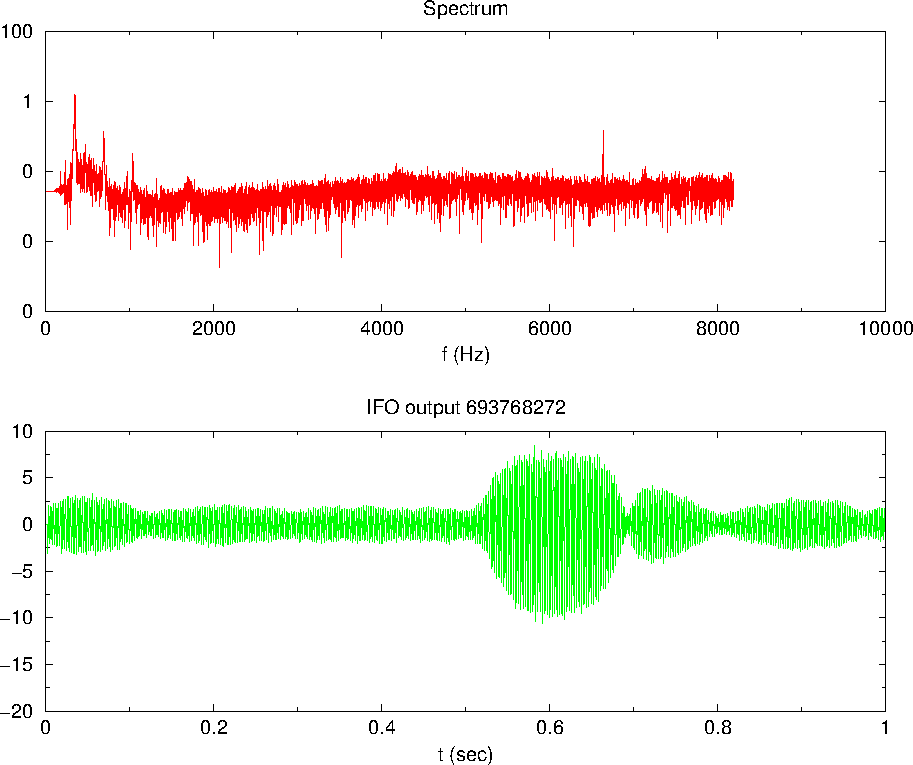
\includegraphics[angle=-90,width=400pt]{animate}
\end{center}
\end{figure}

\item[Author]
Bruce Allen and Patrick Brady

\end{entry}

%%%%%%%%%%%%%%%%%%%%%%%%%%%%%%%%%%%%%%%%%%%%%%%%%%%%%%%%%%%%%%%%%%%%%
%% ZPG2Transfer
%%%%%%%%%%%%%%%%%%%%%%%%%%%%%%%%%%%%%%%%%%%%%%%%%%%%%%%%%%%%%%%%%%%%%
\section{Program \texttt{lalapps\_ZPG2Transfer}}
\label{program:lalapps-ZPG2transfer}
\idx[Program]{lalapps\_ZPG2Transfer}

\begin{entry}

\item[Name]
\verb$lal_ZPG2Transfer$ --- computes transfer function given a
zero-pole-gain representation. 

\item[Synopsis]
\verb$lal_ZPG2Transfer$ [\verb$-z nz z_1 ... z_nz$] [\verb$-p np p_1 .... p_np$] 
                         [\verb$-g gain$] [\verb$-f npoints fmin fmax$] [\verb$-t$]
                         [\verb$-o outfile$] [\verb$-i ilwdfile$]
                         
\item[Description]
\verb$lal_ZPG2Transfer$ computes the frequency domain transfer
function $T(f)$ given a zero-pole-gain representation.   It uses
\verb$LALComputeTransfer()$;  see the LAL Software Documentation under
\texttt{tools} for the definition of the transfer function.

\item[Options]\leavevmode
\begin{entry}
\item[\texttt{-h}]
Print a help message.
\item[\texttt{-z nz z\_1 ... z\_nz}] 
The number of zeros \verb$nz$ followed
by a space and a white space list of \emph{real} zeros specified in units of Hz.
\item[\texttt{-p np p\_1 ... p\_np}] 
The number of zeros \verb$np$ followed
by a space and a white space list of \emph{real} poles specified in units of Hz.
\item[\texttt{-g gain}] 
The gain of the filter.
\item[\texttt{-t}]
If this flag is used,  then the ilwd will indicate units of
counts/attostrain.  The user must correctly choose the zeros, poles,
and gains,  it is not handled automatically.
\item[\texttt{-f npoints fmin fmax}] 
Information about the frequency series.  \verb$npoints$ is the number
of points in the series,  \verb$fmin$ is the lowest frequency to be
represented,  and \verb$fmax$ is the highest frequency to be
represented.   
\item[\texttt{-o} \textit{outfile}]
Write the output to file \textit{outfile} as 3 columns.  Each row
represents the triplet: $\{f,\; \textrm{Re}[T(f)],\; \textrm{Im}[T(f)]\}$.
\item[\texttt{-i} \textit{outfile}]
Write the output to file \textit{outfile} in ILWD format suitable for
ingestion by the datacondAPI in LDAS.
\end{entry}

\item[Example usage]
To compute the transfer function 4 zeros at $0,0,0.74,0.74$Hz,  5
poles at $50.35,50.35,12.1,12.1,186.0$Hz,  and gain $1.47e7$ at 1025
sample points from $0.0$Hz up to $1024.0$Hz and write the ouput as
ILWD:
\begin{verbatim}
./lalapps_ZPG2Transfer -z 4 0.0 0.0 0.74 0.74 \
   -p 5 50.35 50.35 12.1 12.1 186.0 -g 1.47e7 \
   -f 1025 0.0 1024.0 -o response.txt
\end{verbatim}

\item[Author]
Patrick Brady

\end{entry}


%%%%%%%%%%%%%%%%%%%%%%%%%%%%%%%%%%%%%%%%%%%%%%%%%%%%%%%%%%%%%%%%%%%%%
%% BuildTransfer
%%%%%%%%%%%%%%%%%%%%%%%%%%%%%%%%%%%%%%%%%%%%%%%%%%%%%%%%%%%%%%%%%%%%%
\section{Program \texttt{lalapps\_buildTransfer}}
\label{program:lalapps-buildTransfer}
\idx[Program]{lalapps\_buildTransfer}

\begin{entry}

\item[Name]
\verb$lalapps_buildTransfer$ --- computes instrument response function
given a measured swept sine calibration and an overall amplitude
normalization.    

\item[Synopsis]
\verb$lal_buildTransfer$ [\verb$-f npoints fmin fmax$] [\verb$-t$]
                         [\verb$-r outfile$] [\verb$-o outfile$] [\verb$-i ilwdfile$]
                         
\item[Description]
\verb$lal_BuildTransfer$ computes the frequency domain response
function $R(f)$ given a measured swept sine calibration and an overall
amplitude normalization.   

\item[Options]\leavevmode
\begin{entry}
\item[\texttt{-h}]
Print a help message.
\item[\texttt{-r} \textit{infile}]
The input file containing the swept sine calibration.   It should
contain five columns containing frequency, amplitude, error in
amplitude, phase, and error in phase.  See XX for complete
documentation.  
\item[\texttt{-t}]
If this flag is used,  then the ilwd will indicate units of
counts/attostrain.  
\item[\texttt{-f npoints fmin fmax}] 
Information about the frequency series.  \verb$npoints$ is the number
of points in the series,  \verb$fmin$ is the lowest frequency to be
represented,  and \verb$fmax$ is the highest frequency to be
represented.   
\item[\texttt{-o} \textit{outfile}]
Write the output to file \textit{outfile} as 3 columns.  Each row
represents the triplet: $\{f,\; \textrm{Re}[R(f)],\; \textrm{Im}[R(f)]\}$.
\item[\texttt{-i} \textit{outfile}]
Write the output to file \textit{outfile} in ILWD format suitable for
ingestion by the datacondAPI in LDAS.
\end{entry}

\item[Example usage]

To compute the response function from a swept-sine file
\texttt{swept.sine} sample points from $0.0$Hz up to $1024.0$Hz and
write the ouput as ILWD:
\begin{verbatim}
./lalapps_BuildTransfer -z 4 0.0 0.0 0.74 0.74 \
   -p 5 50.35 50.35 12.1 12.1 186.0 -g 1.47e7 \
   -f 1025 0.0 1024.0 -o response.txt
\end{verbatim}

\item[Author]
Patrick Brady

\end{entry}

\section{Stochastic Search Programs}
\label{section:stochastic}

This section of \textsc{LALApps} contains programs that can be used to
search interferometer data for stochastic gravitational wave
backgrounds.

\clearpage
\section{Program \texttt{lalapps\_olapredfcn}}
\label{program:lalapps-olapredfcn}
\idx[Program]{lalapps\_olapredfcn}

\begin{entry}

\item[Name]
%
  \verb$lal_olapredfcn$ --- computes overlap reduction function given
  a pair of known detectors.

\item[Synopsis]
%
  \verb$lal_olapredfcn $[\verb$-h$]\verb$ $[\verb$-q$]\verb$ $[\verb$-v$]
  \verb$ $[\verb$-d debugLevel $]\verb+ \+\newline
  \verb$   $
  \verb$-s siteID1 $[\verb$-a azimuth1$]
  \verb$-t siteID2 $[\verb$-b azimuth2$]\verb+ \+\newline
  \verb$   $
  [\verb$-f fLow$]\verb$ -e deltaF$\verb$ -n numPoints$\verb$ -o outfile$
                         
\item[Description]
%
  \verb$lal_olapredfcn$ computes the overlap reduction function
  $\gamma(f)$ for a pair of known gravitational wave detectors.  It
  uses the LAL function \verb$LALOverlapReductionFunction()$, which is
  documented in the LAL Software Documentation under the
  \texttt{stochastic} package.

\item[Options]\leavevmode
\begin{entry}
\item[\texttt{-h}]
  Print a help message.
\item[\texttt{-q}]
  Run silently (redirect standard input and error to \texttt{/dev/null}).
\item[\texttt{-v}]
  Run in verbose mode.
\item[\texttt{-d} \textit{debugLevel}]
  Set the LAL debug level to \textit{debugLevel}.
\item[\texttt{-s} \textit{siteID1} \texttt{-t} \textit{siteID2}]
  Use detector sites identified by \textit{siteID1} and
  \textit{siteID2}; ID numbers between \texttt{LALNumCachedDetectors}
  (defined in the \texttt{tools} package of LAL) refer to detectors
  cached in the constant array \verb$lalCachedDetectors[]$.  (At this
  point, these are all interferometers.)  Additionally, the five
  resonant bar detectors of the IGEC collaboration can be specified.
  The bar geometry data (summarized in table~\ref{table:cachedBars})
  is used by the fucntion \verb$LALCreateDetector()$ from the
  \texttt{tools} package of LAL to generate the Cartesian position
  vector and response tensor which are used to calculate the overlap
  reduction function.  The ID numbers for the bars depend on the value
  of \texttt{LALNumCachedDetectors}; the correct ID numbers can be
  obtained by with the command
\begin{verbatim}
./lalapps_olapredfcn -h
\end{verbatim}
\item[\texttt{-a} \textit{azimuth1} \texttt{-b} \textit{azimuth2}]
%
  If \textit{siteID1} (\textit{siteID2}) is a bar detector, assume it
  has an azimuth of \textit{azimuth1} (\textit{azimuth2}) degrees East
  of North rather than the default IGEC orientation given in
  table~\ref{table:cachedBars}.  Note that this convention, measuring
  azimuth in degrees clockwise from North is not the same as that used
  in LAL (which comes from the frame spec).  Note also that any
  specified azimuth angle is ignored if the corresponding detector is
  an interferometer.
\item[\texttt{-f} \textit{fLow}]
  Begin the frequency series at a frequency of \textit{fLow}\,Hz; if this
  is omitted, the default value of 0\,Hz is used.
\item[\texttt{-e} \textit{deltaF}]
  Construct the frequency series with a frequency spacing of
  \textit{deltaF}\,Hz
\item[\texttt{-n} \textit{numPoints}]
  Construct a frequency series with \textit{numPoints} points.
\item[\texttt{-o} \textit{outfile}]
  Write the output to file \textit{outfile}.  The format of this file
  is that output by the routine \verb$LALPrintFrequencySeries()$ in
  the \texttt{support} package of LAL, which consists of a header
  describing metadata followed by two-column rows, each containing the
  doublet $\{f,\gamma(f)\}$.
\end{entry}

\begin{table}[tbp]
  \begin{center}
    \begin{tabular}{|c|c|c|c|}
\hline
      Name & Longitude & Latitude & Azimuth
\\ \hline
\verb$AURIGA$ & $11^\circ56'54''$E & $45^\circ21'12''$N & N$44^\circ$E 
\\ \hline
\verb$NAUTILUS$ & $12^\circ40'21''$E & $41^\circ49'26''$N & N$44^\circ$E 
\\ \hline
\verb$EXPLORER$ & $6^\circ12'$E & $46^\circ27'$N & N$39^\circ$E 
\\ \hline
\verb$ALLEGRO$ & $91^\circ10'43.\!\!''766$W & $30^\circ24'45.\!\!''110$N 
& N$40^\circ$W
\\ \hline
\verb$NIOBE$ & $115^\circ49'$E & $31^\circ56'$S & N$0^\circ$E 
\\ \hline
    \end{tabular}
    \caption{Location and orientation data for the five IGEC resonant
      bar detectors, stored in the \texttt{lalCachedBars[]}
      array.  The data are taken from
      \texttt{http://igec.lnl.infn.it/cgi-bin/browser.pl?Level=0,3,1}
      except for the latitude and longitude of ALLEGRO, which were
      taken from Finn \& Lazzarini, gr-qc/0104040.  Note that the
      elevation above the WGS-84 reference ellipsoid and altitude
      angle for each bar is not given, and therefore set to zero.}
    \label{table:cachedBars}
  \end{center}
\end{table}


\item[Example usage]
  To compute the overlap reduction function for LIGO Hanford and
  LIGO Livingston, with a resolution of 1\,Hz from 0\,Hz to 1024\,Hz:
\begin{verbatim}
lalapps_olapredfcn -s 0 -t 1 -e 1 -n 1025 -o LHOLLO.dat
\end{verbatim}
  
  To compute the overlap reduction function for ALLEGRO in its optimal
  orientation of $72.\!\!^\circ08$ West of South (see Finn \& Lazzarini,
  gr-qc/0104040) and LIGO Livingston, with a resolution of 0.5\,Hz from
  782.5\,Hz to 1032\,Hz (assuming \texttt{lalNumCachedBars} is 6):
\begin{verbatim}
lalapps_olapredfcn -s 9 -a 252.08 -t 1 -f 782.5 -e 0.5 -n 500 -o ALLEGROLHO.dat
\end{verbatim}

\item[Author]
John T.~Whelan

\end{entry}


\clearpage
\subsection{Program \texttt{lalapps\_stochastic\_pipe}}
\label{program:stochastic-pipeline}
\idx[Program]{stochastic\_pipeline.py}

\begin{entry}
\item[Name]
\verb$lalapps_stochastic_pipe$ --- python script to generate Condor DAGs
to run the stochastic pipeline.

\item[Synopsis]
\begin{verbatim}
  -h, --help               display this message
  -v, --version            print version information and exit

  -d, --datafind           run LSCdataFind to create frame cache files
  -s, --stochastic         run lalapps_stochastic

  -p, --playground-only    only create chunks that overlap with playground
  -P, --priority PRIO      run jobs with condor priority PRIO

  -f, --config-file FILE   use configuration file FILE
  -l, --log-path PATH      directory to write condor log file
\end{verbatim}

\item[Description] \verb$lalapps_stochastic_pipe$ generates a Condor DAG
to run the stochastic search pipeline. The configuration should specify
the parameters needed to run the jobs and must be specified with the
\verb$--config-file$ option. A file containing science segments to
analysed should be specified in the \verb$[input]$ section of the
configuration file with a line such as
\begin{verbatim}
segments = S2H1L1v03_selectedsegs.txt
\end{verbatim}
This should contain four whitespace separated columns:
\begin{verbatim}
  segment_id    gps_start_time    gps_end_time    duration
\end{verbatim}
that define the science segments to be used. Lines starting with an
octothorpe are ignored.

\item[Example]
Generate a DAG to run a stochastic search on a pair of interferometers
specified in the configuration file. The generated DAG is then submitted
with \texttt{condor\_submit\_dag}
\begin{verbatim}
lalapps_inspiral_pipe --log-path /home/ram/dag_logs \
--datafind --stochastic --config-file stochastic_H1L1.ini

condor_submit_dag stochastic_H1L1.dag
\end{verbatim}

\item[Author]
Adam Mercer
\end{entry}

\clearpage
\subsection{Program \texttt{lalapps\_stochastic}}
\label{program:lalapps-stochastic}
\idx[Program]{lalapps\_stochastic}

\begin{entry}
\item[Name]
\verb$lalapps_stochastic$ --- standalone stochastic analysis code.

\item[Synopsis]
\begin{verbatim}
 --help                        print this message
 --version                     display version
 --verbose                     verbose mode
 --debug-level LEVEL           set lalDebugLevel
 --gps-start-time SEC          GPS start time
 --gps-end-time SEC            GPS end time
 --segment-duration SEC        segment duration
 --resample-rate F             resample rate
 --f-min F                     minimal frequency
 --f-max F                     maximal frequency
 --hann-duration SEC           hann duration
 --ifo-one IFO                 ifo for first stream
 --ifo-two IFO                 ifo for second stream
 --data-cache-one FILE         cache file for first stream
 --data-cache-two FILE         cache file for second stream
 --calibration-cache-one FILE  first stream calibration cache
 --calibration-cache-two FILE  second stream calibration cache
 --apply-mask                  apply frequency masking
 --inject                      inject a signal into the data
 --scale-factor N              scale factor for injection
 --seed N                      seed
 --overlap-hann                overlaping hann windows for data windowing
 --high-pass-filter            perform high pass filtering
\end{verbatim}

\item[Description] \verb$lalapps_stochastic$ runs the standalone
stochastic analysis code.

\item[Author] 
Adam Mercer, Tania Regimbau
\end{entry}

\chapter{Package \texttt{ring}}

\newpage\input{RingH}
\newpage\input{LALRingDownH}
\newpage\input{LALWienerH}

\newpage\begin{thebibliography}{0}
\bibitem{EWLeaver}
  E. W. Leaver, Proc. R. Soc. London \textbf{A402}, 285 (1985).
\bibitem{FEcheverria}
  F. Echeverria, Phys. Rev. D \textbf{40}, 3194 (1989).
\bibitem{BJOwen}
  B. J. Owen, Phys. Rev. D \textbf{53}, 6749 (1996).
\bibitem{JDECreighton}
  J. D. E. Creighton, Phys. Rev. D \textbf{60}, 022001 (1999).
\end{thebibliography}


\section{Program \texttt{lalapps\_inspinj}}
\label{program:lalapps-inspinj}
\idx[Program]{lalapps\_inspinj}

\begin{entry}
\item[Name]
\verb$lalapps_inspinj$ --- produces inspiral injection data files.

\item[Synopsis]
\verb$lalapps_inspinj$ \newline
%
[\texttt{--help}]\newline
\texttt{--source-file} \textsc{sfile} \newline
\texttt{--mass-file} \textsc{mfile}\newline
%
[\texttt{--gps-start-time} \textsc{tstart}]\newline 
[\texttt{--gps-end-time} \textsc{tend}]\newline
%
[\texttt{--time-step} \textsc{tstep}] \newline
[\texttt{--time-interval} \textsc{tinterval}]\newline
%
[\texttt{--seed} \textsc{seed}]\newline
[\texttt{--waveform} \textsc{wave}]\newline
[\texttt{--usertag} \textsc{tag}]\newline
%
[\texttt{--tama-output}]\newline
[\texttt{--ilwd}]

\item[Description] 
\verb$lalapps_inspinj$
generates a number of inspiral  parameters suitable  for using in a Monte
Carlo injection to test the efficiency of a inspiral search.  The  various
parameters (detailed  below)  are randomly chosen and are appropriate for a
particular population of binary neutron stars  whose spatial  distribution
includes the Milky Way and a number of extragalactic objects that are  input
in  a  datafile.  The  possible  mass pairs for the binary neutron star com-
panions are also specified in a (different) datafile.

The output of this program  is  a  list  of  the  injected events,  starting
at  the specified start time and ending at the specified end time.  One 
injection with random inspiral parameters will be made every specified time
step, and will be randomly placed within the specified time interval.  
The output is written to a file name in the standard inspiral pipeline format:
\begin{center}
\begin{verbatim}
HL-INJECTIONS_USERTAG_SEED-GPSSTART-DURATION.xml
\end{verbatim}
\end{center}
where \verb$USERTAG$ is \textsc{tag} as specfied on the command line, 
\verb$SEED$ is the  value  of  the random number seed chosen and 
\verb$GPSSTART$ and \verb$DURATION$ describes the GPS time interval that
the file covers. The file is in the standard LIGO lightweight XML format
containing a \texttt{sim\_inspiral} table that describes the injections.
In addition, an ASCII log file called \verb$injlog.txt$ is also written.
If a \texttt{--user-tag} is not specified on the command line, the
\texttt{\_USERTAG} part of the filename will be omitted.

\item[Options]\leavevmode
\begin{entry}
\item[\texttt{--help}] Print a help message.

\item[\texttt{--source-file} \textsc{sfile}]
Optional. Data file containing spatial distribution of  extragalactic  objects.
Default  is  the file \verb+inspsrcs.dat+ provided by LALApps. If that file is 
empty, all signals are in the Milky Way.

\item[\texttt{--mass-file} \textsc{mfile}]
Optional. Data file containing mass pairs  for  the binary  neutron  star
companions.   Default is the file \verb+BNSMasses.dat+ provided by LALApps.

\item[\texttt{--gps-start-time} \textsc{tstart}]
Optional.  Start time of the injection data to be created. Defaults to the
start of S2, Feb 14 2003 16:00:00 UTC (GPS time 729273613)

\item[\texttt{--gps-end-time} \textsc{tend}]
Optional. End time of the injection data to be created. Defaults to the end of
S2, Apr 14 2003 15:00:00 UTC (GPS time 734367613).

\item[\texttt{--time-step} \textsc{tstep}]
Optional. Sets the time step interval between injections. The injections will
occur with an average spacing of \textsc{tstep} seconds. Defaults to 
$2630/\pi$.

\item[\texttt{--time-interval} \textsc{tinterval}]
Optional. Sets the time interval during which an injection can occur. 
Injections are uniformly distributed over the interval.  Setting \textsc{tstep}
to $6370$ and \textsc{tinterval} to 600 guarantees there will be one injection
into each playground segment and they will be randomly distributed within the
playground times.

\item[\texttt{--seed} \textsc{seed}]
Optional. Seed the random number generator with the integer \textsc{seed}.
Defaults to $1$.

\item[\texttt{--waveform} \textsc{wave}]
Optional. The string \textsc{wave} will be written into the \texttt{waveform}
column of the \texttt{sim\_inspiral} table output. This is used by the
inspiral code to determine which type of waveforms it should inject into the
data. Defaults is \texttt{GeneratePPNtwoPN}.

\item[\texttt{--user-tag} \textsc{string}] Optional. Set the user tag for this
job to be \textsc{string}. May also be specified on the command line as 
\texttt{-userTag} for LIGO database compatibility.

\item[\texttt{--tama-output}]
Optional.  If this option is given, \verb+lalapps_inspinj+ also produces a 
text output file:
\begin{center}
\begin{verbatim}
HLT-INJECTIONS_USERTAG_SEED-GPSSTART-DURATION.txt
\end{verbatim}
\end{center}
which contains the following fields:

\begin{itemize}
\item geocentric end time
\item Hanford end time
\item Livingston end time
\item Tama end time
\item total mass, $M_{\mathrm{TOT}}$
\item mass ratio, $\eta$
\item distance to source (in Mpc)
\item longitude
\item latitude
\item inclination
\item coalescence phase
\item polarization
\end{itemize}

In the above, all times are recorded as double precision real numbers and all
angles are in radians.  

\item[\texttt{--ilwd}] Optional. If this option is given,
\verb+lalapps_inspinj+ also produces two ILWD-format files, injepochs.ilwd and
injparams.ilwd, that contain, respectively, the  GPS  times  suitable for
inspiral injections, and the intrinsic inspiral signal parameters to be used
for  those injections.

The  file  injepochs.ilwd  contains  a sequence of integer pairs representing
the injection GPS time in  seconds  and residual  nano-seconds.   The file
injparams.ilwd contains the intrinsic binary parameters for each injection,
which is  a  sequence  of  eight  real  numbers representing (in order) (1) the
total mass of the binary system  (in  solar masses),  (2)  the  dimensionless
reduced mass --- reduced mass per unit total mass --- in the range from  0
(extreme mass  ratio)  to  0.25 (equal masses), (3) the distance to the system
in meters, (4) the inclination  of  the  binary system  orbit  to the plane of
the sky in radians, (5) the coalescence phase in radians, (6)  the  longitude
to  the direction  of  the  source in radians, (7) the latitude to the
direction of the source in radians, (8) and the polar- ization angle of the
source in radians.
\end{entry}

\item[Example]
\begin{verbatim}
lalapps_inspinj --seed 45\
--source-file inspsrcs.dat --mass-file BNSMasses.dat
\end{verbatim}

\item[Environment]\leavevmode
\begin{entry}
\item[LALAPPS\_DATA\_PATH] Directory to look for the default mass
file \verb+BNSMasses.dat+ and the default source file \verb+inspsrcs.dat+.
\end{entry}


\item[Author] 
Jolien Creighton, Patrick Brady, Duncan Brown
\end{entry}



\section{Program \texttt{lalapps\_findchirp\_post}}
\label{program:lalapps-findchirp-post}
\idx[Program]{lalapps\_findchirp\_post}

\begin{entry}

\item[Name]
\verb$lalapps_findchirp_post$ --- post process event files from findchirp

\item[Synopsis]
\verb$lalapps_inspinj$ [\verb$-h$] [\verb$-V$] [\verb$-v$]
[\verb$-d$ \textit{dbglvl}]
[\verb$-m$]
[\verb$-s$ \textit{minsnr}\texttt{-}\textit{maxsnr}]
[\verb$-c$ \textit{minchisq}\texttt{-}\textit{maxchisq}]
[\verb$-b$ \textit{bins}]
[\verb$-e$ \textit{eventfile}]

\item[Description]

\verb$lalapps_inspinj$ post process event files from findchirp.

\item[Options]\leavevmode
\begin{entry}
\item[\texttt{-h}]
Print a help message.
\item[\texttt{-V}]
Print the version information.
\item[\texttt{-v}]
Verbose output.
\item[\texttt{-d} \textit{dbglvl}]
Set LAL debug level to \textit{dbglvl}.
\item[\texttt{-m}]
Maximize events over injections. This options caused only the loudest event
(in SNR) in each window of length $100/\pi = 31.8309886183791$ to be processed.
The window starts at the time of the first event.
\item[\texttt{-s} \textit{minsnr}\texttt{-}\textit{mmaxsnr}]
Set minimum and maximum of the range of signal to noise ratio for creation
of the histogram bins.  (Default is 7.0\-14.0.)
\item[\texttt{-c} \textit{minchisq}\texttt{-}\textit{mmaxchisq}]
Set minimum and maximum of the range of chi squared veto statistic for
creation of the histogram bins.  (Default is 0.0\-50.0.)
\item[\texttt{-b} \textit{bins}]
Set the number of bins in the two dimensional histogram. (Default is 10.)
\item[\texttt{-e} \textit{eventfile}]
Set the path to the file containing the list of inspiral events. 
(Default is \verb|eventfile.dat|.) The event file must be of the format
\verb|END_TIME END_TIME_NS EFF_DISTANCE MASS1 MASS2 MCHIRP ETA SNR CHISQ SIGMASQ|.
Each event should be separated by a new line. Lines beginning with an
octothorpe are ignored.
\end{entry}

\item[Debug levels]
The LAL debug level can be specified as an integer or as a string of flags:
\begin{entry}
\item[\texttt{NDEBUG}]
No debugging information is printed and memory debugging code is disabled.
\item[\texttt{ERROR}]
Error messages are printed.
\item[\texttt{WARNING}]
Warning messages are printed.
\item[\texttt{INFO}]
Information messages are printed.
\item[\texttt{TRACE}]
Function call tracing messages are printed.
\item[\texttt{MEMINFO}]
Memory  allocation  information messages are printed.
\item[\texttt{MEMDBG}]
Debugging of memory allocation routines is enabled but no messages are printed.
\end{entry}
The following composite levels are available:
\begin{entry}
\item[\texttt{MSGLVL1}]
Equivalent to \verb$ERROR$
\item[\texttt{MSGLVL2}]
Equivalent to \verb$ERROR | WARNING$
\item[\texttt{MSGLVL3}]
Equivalent to \verb$ERROR | WARNING | INFO$
\item[\texttt{ALLDBG}]
All debugging messages are printed.
\end{entry}

For example, the command
\begin{indented}
\verb$lalapps_inspinj -d "ERROR | INFO"$
\end{indented}
will set the debug level so that error and information messages are printed.

\item[Environment]\leavevmode

\begin{entry}
\item[\texttt{LAL\_DEBUG\_LEVEL}]
Default LAL debug level to use.
\end{entry}

\item[Author]
Duncan Brown

\end{entry}



\backmatter

\nocite{*}
\bibliography{lalapps}

\printindex

\end{document}
